Zur Dekodierung auf eine bestimmte Lautsprecheranordnung wird eine Matrix aus virtuellen Mikrofonen berechnet, woraus sich eine Tabelle mit Gain-Werte ergibt. Diese Tabelle kann die einzelne Frequenzbins in einem VBAP-Verfahren den enstprechenden Lautsprechern zuordnen. In dieser Seminararbeit wurden dabei zwei Ansätze für die Dekodierung verglichen: Einerseits die direkte Dekodierung auf die Lautsprecheranordnung des widergebenden Systems, und andererseits ein eher allgemeiner Ansatz womit die Dekodierung auf ein ambisonisches B-Format Array vierter Ordnung erfolgt. Dieser Dekodierungsansatz hat den Vorteil, dass die Wiedergabeanordnung zum Zeitpunkt des Upmixings nicht vorgegeben sein muss. Auch für die Klangqualität stellen sich hierdurch Vorteile heraus welche im Hörversuch besprochen werden.

Die Dekodierung auf eine gegebene Lautsprecheranordnung durch eine VBAP-Tabelle wird hier nicht weiter ausgeführt und kann zum Beispiel im Buch "Ambisonics" \ref{} nachgelesen werden. Für das B-Format vierter Ordnung wird ein sogenanntes T-Design als virtuelle Anordnung von Lautsprechern verwendet. Ein T-Design ist grundsätzlich zur Darstellung der Maxima von sphärischen Harmonischen notwendig. Wird ein T-Design neunter Ordnung eingesetzt ("9-Design", Abb. \ref{fig:tdesign}) ergibt sich daraus eine sphärische Anordnung von 48 Lautsprechern, welche die verlustlose Konvertierung zwischen B-Format und einer solchen Lautsprecheranordnung bietet. Es lässt sich sagen, dass ein 9-Design dem ambisonischen B-Format vierter Ordnung entspricht.

\begin{figure}[!ht]
  \centering
  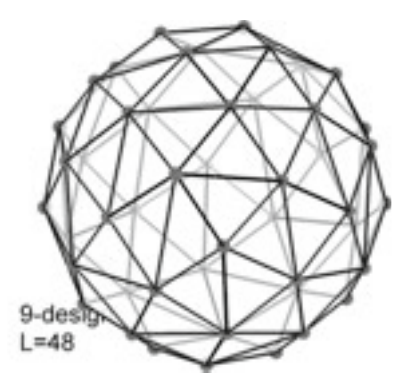
\includegraphics[width=0.35\textwidth]{implementierung/plots/t-design.png}
  \label{fig:tdesign}
  \caption{9-Design T-Design\protect\footnotemark}
\end{figure}

\footnotetext{Quelle: \cite{ambi-book}}

Zur Dekodierung wird in Octave also eine Matrix mit Lautsprecheramplituden für Schalleinfallsrichtungen erstellt. Somit kann einer gegebenen Richtung (bestehend aus Azimuth und Elevation) eine Amplitude am entsprechenden Lautsprecherkanal zugeordnet werden.
